% $Header: /cvsroot/latex-beamer/latex-beamer/solutions/conference-talks/conference-ornate-20min.en.tex,v 1.6 2004/10/07 20:53:08 tantau Exp $

\documentclass{beamer}
%\documentclass[handout]{beamer}
%\usepackage{pgfpages}
%\pgfpagesuselayout{2 on 1}[a4paper,border shrink=5mm]

% This file is a solution template for:

% - Talk at a conference/colloquium.
% - Talk length is about 20min.
% - Style is ornate.



% Copyright 2004 by Till Tantau <tantau@users.sourceforge.net>.
%
% In principle, this file can be redistributed and/or modified under
% the terms of the GNU Public License, version 2.
%
% However, this file is supposed to be a template to be modified
% for your own needs. For this reason, if you use this file as a
% template and not specifically distribute it as part of a another
% package/program, I grant the extra permission to freely copy and
% modify this file as you see fit and even to delete this copyright
% notice.


\mode<presentation>
{
%  \usetheme{Warsaw}
%  \usetheme{Boadilla}
%  \usetheme{Goettingen}
%  \usetheme{Hannover}
%  \usetheme{Madrid}
%  \usetheme{Marburg}
%  \usetheme{Montpellier}
%  \usetheme{Pittsburgh}
  \usetheme{Hawke}
  % or ...

  \setbeamercovered{transparent}
  % or whatever (possibly just delete it)
}


\usepackage[english]{babel}
% or whatever

\usepackage[latin1]{inputenc}
% or whatever

\usepackage{times}
\usepackage[T1]{fontenc}
% Or whatever. Note that the encoding and the font should match. If T1
% does not look nice, try deleting the line with the fontenc.

\usepackage{multimedia}


%%%%%%
% My Commands
%%%%%%

\newcommand{\ml}{{\sc matlab}}
\newcommand{\bb}{{\boldsymbol{b}}}
\newcommand{\bx}{{\boldsymbol{x}}}
\newcommand{\by}{{\boldsymbol{y}}}
\newcommand{\bfm}[1]{{\boldsymbol{#1}}}

%%%%

\title[Lecture 12] % (optional, use only with long paper titles)
{Lecture 12 - Quadrature}

% \subtitle
% {Include Only If Paper Has a Subtitle}

\author[I. Hawke] % (optional, use only with lots of authors)
{I.~Hawke}
% - Give the names in the same order as the appear in the paper.
% - Use the \inst{?} command only if the authors have different
%   affiliation.

\institute[University of Southampton] % (optional, but mostly needed)
{
%  \inst{1}%
  School of Mathematics, \\
  University of Southampton, UK
}
% - Use the \inst command only if there are several affiliations.
% - Keep it simple, no one is interested in your street address.

\date[Semester 1] % (optional, should be abbreviation of conference name)
{MATH3018/6141, Semester 1}
% - Either use conference name or its abbreviation.
% - Not really informative to the audience, more for people (including
%   yourself) who are reading the slides online

\subject{Numerical methods}
% This is only inserted into the PDF information catalog. Can be left
% out.



% If you have a file called "university-logo-filename.xxx", where xxx
% is a graphic format that can be processed by latex or pdflatex,
% resp., then you can add a logo as follows:

\pgfdeclareimage[height=0.5cm]{university-logo}{mathematics_7469}
\logo{\pgfuseimage{university-logo}}



% Delete this, if you do not want the table of contents to pop up at
% the beginning of each subsection:
%  \AtBeginSubsection[]
%  {
%    \begin{frame}<beamer>
%      \frametitle{Outline}
%      \tableofcontents[currentsection,currentsubsection]
%    \end{frame}
%  }
\AtBeginSection[]
{
  \begin{frame}<beamer>
    \frametitle{Outline}
    \tableofcontents[currentsection]
  \end{frame}
}


% If you wish to uncover everything in a step-wise fashion, uncomment
% the following command:

%\beamerdefaultoverlayspecification{<+->}


\begin{document}

\begin{frame}
  \titlepage
\end{frame}

\section{Simpson's Rule}

\subsection{Simpson's Rule}

\begin{frame}
  \frametitle{Improving Convergence}

  The aim of numerical quadrature is to compute
  \begin{equation*}
    \int_a^b f(x) \, \text{d}x
  \end{equation*}
  where $f$ is a real function of a single variable $x$.

  \vspace{1ex}

  Simple methods use polynomial quadrature: function values known
  at \emph{nodes} are interpolated by a (piecewise) polynomial $g$. The
  quadrature is approximated by $\int g(x) \, \text{d}x$. \pause

  \vspace{1ex}

  Introduced (composite) \emph{trapezoidal} rule, where $g$ is a
  (piecewise) linear polynomial -- a straight line connecting
  neighbouring nodes. \pause

  \vspace{1ex}

  Can improve accuracy by increasing the order of $g$.  Simplest
  improvement uses a quadratic polynomial, giving \emph{Simpson's}
  rule.

\end{frame}

\begin{frame}
  \frametitle{Simpson's rule}

  \begin{columns}
    \begin{column}{0.5\textwidth}
      Three points are needed to determine a unique polynomial of
      order two. Our discussion of Simpson's rule will always assume
      equally spaced points, so on the interval $[a, b]$ we use $\{a,
      (a+b)/2, b\}$ with $h = (b-a)/2$. \pause

      \vspace{1ex}

      Work in coordinates about the centre of the interval, $\hat{x} =
      x - (a+b)/2$. Hence $\hat{x} \in [-h, h]$.
    \end{column}
    \begin{column}{0.5\textwidth}
      \begin{center}
        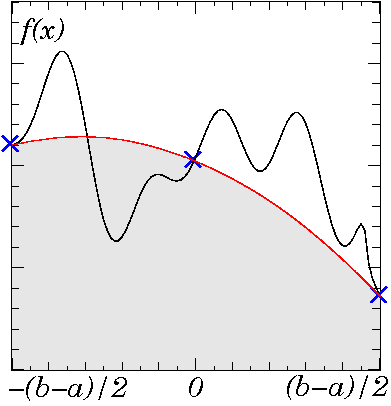
\includegraphics[width=\textwidth]{figures/SimpsonNodes}
      \end{center}
    \end{column}
  \end{columns}


\end{frame}

\begin{frame}
  \frametitle{Interpolating polynomial}

  In the coordinates $\hat{x} = x - (a+b)/2$ we have
  \begin{align*}
    && g(\hat{x}) & = \alpha \hat{x}^2 + \beta \hat{x} + \gamma, &
    \hat{x} \in [-h, h] \\
    \Rightarrow && A & = \int_{-h}^h g(\hat{x}) \, \text{d}x \\
    &&& = \tfrac{\alpha}{3} \left( 2 h^3 \right) + \gamma \left( 2 h
    \right).
  \end{align*} \pause
%
  Simple to evaluate the coefficients as
  \begin{align*}
    g(\hat{x} = 0) & = \gamma, \\
    g(\hat{x} = -h) + g(\hat{x} = h) & = 2 \alpha h^2 + 2 \gamma.
  \end{align*} \pause
%
  Putting this together we have
  \begin{align*}
    A & = \tfrac{h}{3} \left( \left( 2 \alpha h^2 + 2 \gamma \right) +
      4 \gamma \right) \\
    & = \frac{b - a}{6} \left[ f(a) + 4 f \left( \frac{a + b}{2}
      \right) + f(b) \right].
  \end{align*}

\end{frame}

\begin{frame}
  \frametitle{Composite Simpson's Rule}

  \begin{columns}
    \begin{column}{0.5\textwidth}
      \begin{overlayarea}{\textwidth}{0.8\textheight}
        \only<1|handout:1>
        {
          As with trapezoidal rule, basic Simpson's rule is
          very inaccurate.
        }
        \only<2-|handout:2>
        {
          Instead use the \emph{composite}
          Simpson's rule.  Interval is divided into $N / 2$
          equal subintervals length $2 h$,
          \begin{equation*}
            h = (b - a) / N,
          \end{equation*}
          and Simpson's rule is applied to each subinterval.
        }
        \only<3|handout:2>
        {

          \vspace{1ex}
          The factor of 2 implies 3 nodes in each
          subinterval: the boundary points and a centre point. Each
          subinterval has a unique interpolating quadratic, and no
          quadratic overlaps, giving a simple piecewise polynomial.
        }
      \end{overlayarea}
    \end{column}
    \begin{column}{0.5\textwidth}
      \begin{overlayarea}{\textwidth}{0.7\textheight}
        \only<1|handout:1>
        {
          \begin{center}
            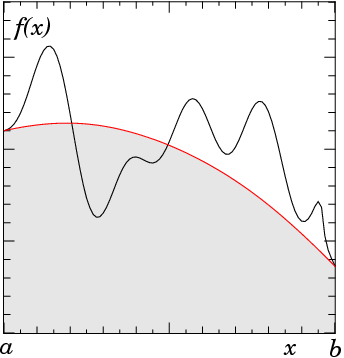
\includegraphics[width=\textwidth]{figures/simpson1}
          \end{center}
        }
        \only<2-|handout:2>
        {
          \begin{center}
            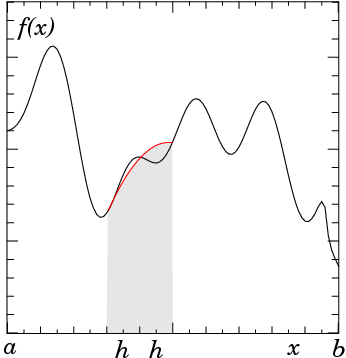
\includegraphics[width=\textwidth]{figures/simpson2}
          \end{center}
        }
      \end{overlayarea}
    \end{column}
  \end{columns}

\end{frame}

\begin{frame}
  \frametitle{Composite Simpson's rule formula}

  With the evenly spaced grid we obtain the formula
  \begin{equation*}
    \int_a^b f(x) \, \text{d}x \simeq \frac{h}{3} \left[ f(a) + f(b) +
      2 \sum_{j=1}^{N/2 - 1} f_{2 j} + 4 \sum_{j=1}^{N/2} f_{2 j - 1}
    \right].
  \end{equation*}
  The error from Simpson's rule is
  \begin{equation*}
    \text{Error} \leq \frac{M_4}{180} ( b - a ) h^4, \quad M_4 = \max
    | f^{(4)} (x) |.
  \end{equation*}

\end{frame}


\subsection{Error analysis}

\begin{frame}
  \frametitle{Errors: 1}

  We find the error by bounding the error for a single interval.
  Write Simpson's rule as a power law expansion in terms of the width
  of the interval $2 h$ with centre $x_j$, and compare to the exact
  solution expansion. \pause

  \vspace{1ex}

  For one interval of Simpson's rule:
  \begin{equation*}
    A_j = \frac{h}{3} \left[ f_{j-1} + 4 f_j + f_{j+1} \right].
  \end{equation*}
  Taylor expand about the centre point of the interval $x_j$:
  \begin{equation*}
    A_j = 2 h f_j + \frac{h^3}{3} f^{(2)}_j + \frac{h^5}{36} f^{(4)}_j
    + {\cal O}(h^6).
  \end{equation*}

\end{frame}

\begin{frame}
  \frametitle{Errors: 2}

  As before we need the exact result in powers of $h$. Working about
  the centre of the interval we define
  \begin{equation*}
    F(t) = \int_{x_j - t}^{x_j + t} f(x) \, \text{d}x
  \end{equation*}
  so that
  \begin{equation*}
    F(h) = \int_{x_{j-1}}^{x_{j+1}} f(x) \, \text{d}x.
  \end{equation*}
  We note that
  \begin{equation*}
    \frac{\text{d}^n F}{\text{d}t^n} = f^{(n-1)}(x_j + t) + (-1)^{n-1}
    f^{(n-1)}(x_j - t)
  \end{equation*}
  or in particular
  \begin{equation*}
    \frac{\text{d} F}{\text{d}t} = f(x_j + t) + f(x_j - t).
  \end{equation*}
\end{frame}


\begin{frame}
  \frametitle{Errors: 3}

  From this we can Taylor expand about $t=0$ to find
  \begin{equation*}
    F(h) = F(0) + h \left. \frac{\text{d}F}{\text{d}t} \right|_{t=0}
    + \dots
  \end{equation*} \pause
  From the definition of $\text{d}F / \text{d}t$ we have
  \begin{equation*}
    F(h) = 2 h f_j + \tfrac{h^3}{3} f^{(2)}_j + \tfrac{h^5}{60}
    f^{(4)}_j + \dots.
  \end{equation*} \pause
  Comparing with Simpson's rule
  \begin{equation*}
    F(h) \simeq A_j = 2 h f_j + \tfrac{h^3}{3} f^{(2)}_j +
    \tfrac{h^5}{36} f^{(4)}_j + \dots
  \end{equation*}
  the error in the subinterval is
  \begin{equation*}
    | A_j - F(h) | \leq \tfrac{h^5}{90} | f^{(4)}_j |.
  \end{equation*} \pause

  Summing over all $N / 2$ subintervals and using $h N = (b - a)$ gives
  \begin{equation*}
    \text{Error} \leq \frac{(b - a) h^4}{180} M_4, \quad M_4 =
    \max_{x\in[a,b]} | f^{(4)}(x) |.
  \end{equation*}

\end{frame}

\subsection{Example}

\begin{frame}
  \frametitle{Example}

  We look at
  \begin{equation*}
    \int_0^{\pi / 2} \sin(x) \, \text{d}x
  \end{equation*}
  using Simpson's rule. The exact answer is 1.

  \begin{overlayarea}{\textwidth}{0.7\textheight}
    \only<2|handout:1>
    {
       With three points $x_j = \{0, \pi / 4, \pi / 2\}$ we have $h =
       \pi / 4$ and
       \begin{center}
         \begin{tabular}{c|c c}
           $j$ & $x_j$ & $f_j$ \\ \hline
           0 & 0 & 0 \\
           1 & $\pi / 4$ & $1 / \sqrt{2}$ \\
           2 & $\pi / 2$ & 1
         \end{tabular}
       \end{center}
       So
       \begin{align*}
         \int_0^{\pi / 2} \sin(x) \, \text{d}x & \simeq \frac{\pi / 4}{3}
         \left( 0 + 1 \right) + \frac{4 (\pi / 4)}{3} \left(
           \tfrac{1}{\sqrt{2}} \right)
         \\
         & = \tfrac{\pi}{12} \left( 1 + 2 \sqrt{2} \right) \\
         & \simeq 1.002.
       \end{align*}
    }
    \only<3|handout:2>
    {
      With five points $x_j = \{0, \pi / 8, \pi / 4, 3 \pi / 8, \pi /
      2\}$ we have
      $h = \pi / 8$ and
      \begin{center}
        \begin{tabular}{c|c c}
          $j$ & $x_j$ & $f_j$ \\ \hline
          0 & 0 & 0 \\
          1 & $\pi / 8$ & $0.38268$ \\
          2 & $\pi / 4$ & $1 / \sqrt{2}$ \\
          3 & $3 \pi / 8$ & $0.92388$ \\
          4 & $\pi / 2$ & 1
        \end{tabular}
      \end{center}
%
      \begin{align*}
        \int_0^{\pi / 2} \sin(x) \, \text{d}x  \simeq \frac{\pi / 8}{3}
        \left( 0 + 1 \right) &+ \frac{4 ( \pi / 8)}{3} \left( 0.38268
          + 0.92388 \right) \\ &+ \frac{2 ( \pi / 8)}{3} \left(
          1 / \sqrt{2} \right) \quad \simeq 1.000135.
      \end{align*}
    }
  \end{overlayarea}

\end{frame}

\begin{frame}
  \frametitle{Example Convergence}

  \begin{center}
    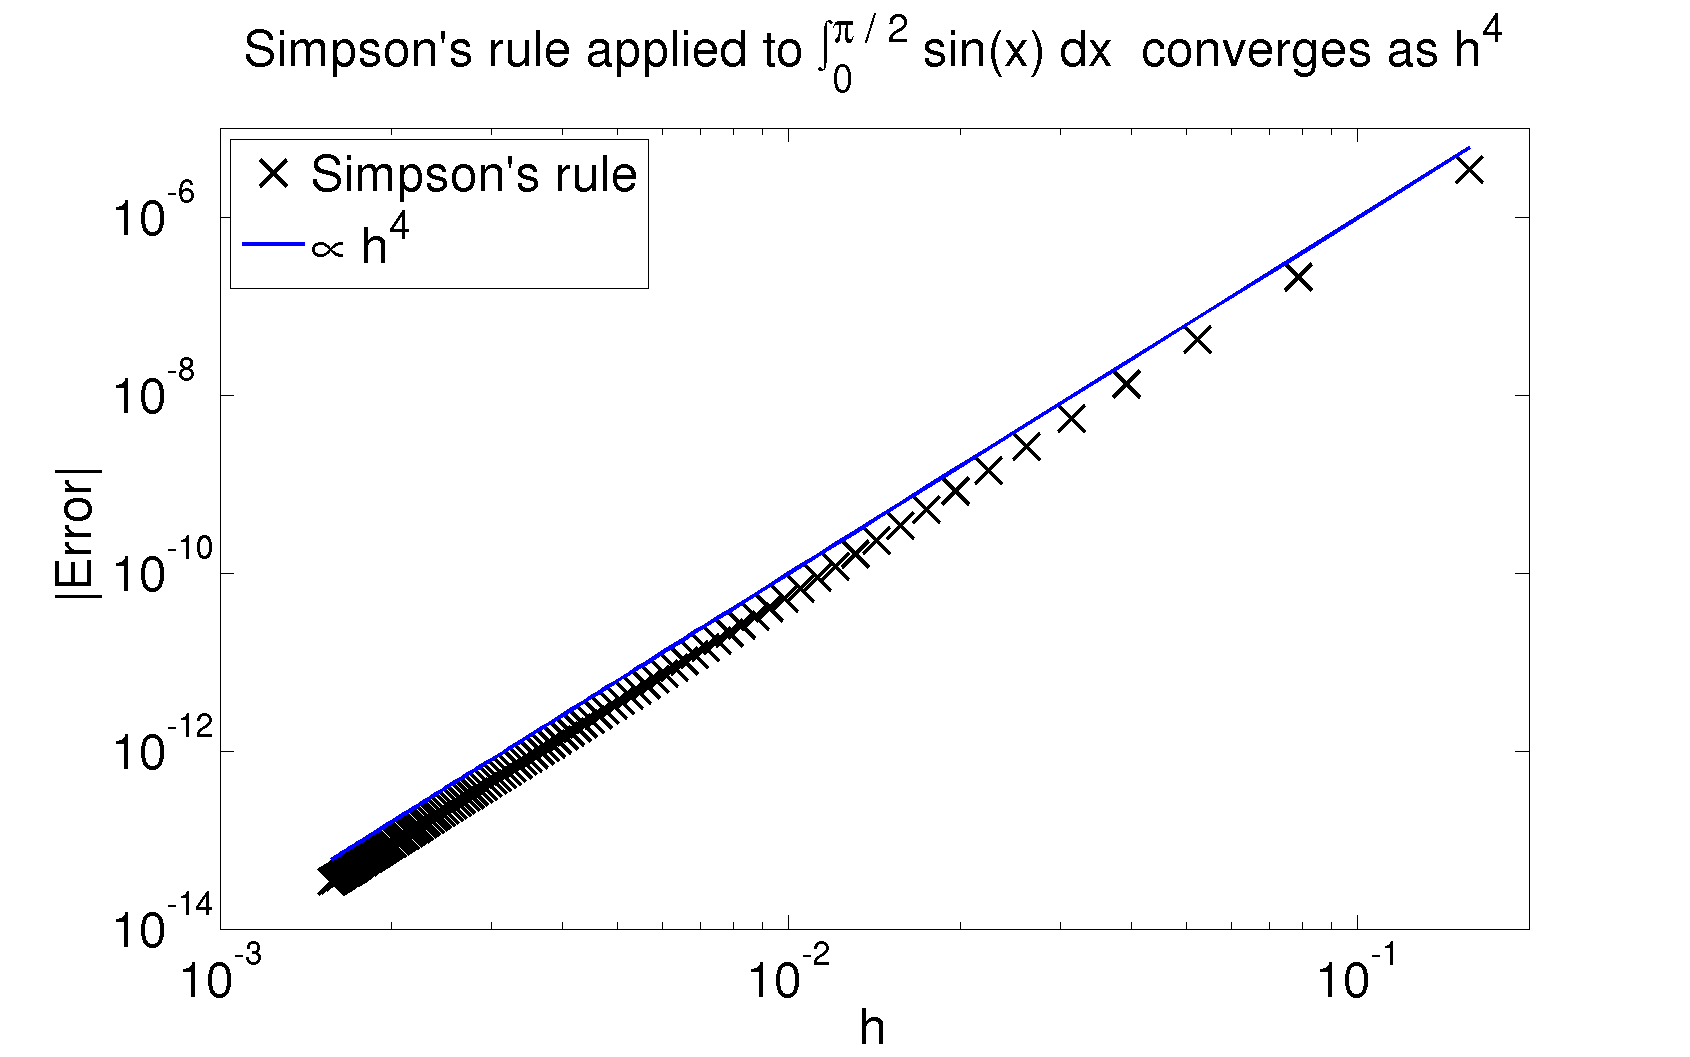
\includegraphics[width=0.8\textwidth]{figures/SimpsonExample1}
  \end{center}
  The example converges as expected with resolution.

\end{frame}


\subsection{Yet higher order}

\begin{frame}
  \frametitle{Yet higher order}

  Why not use cubics, quartics, \dots? \pause

  \vspace{2ex}

  \begin{columns}
    \begin{column}{0.475\textwidth}
      One way of deriving \emph{spectral} methods, which converge
      faster than any polynomial. \pause

      \vspace{1ex}

      \emph{However}, care is required. With equally spaced nodes may
      see problems, e.g.\ the \emph{Runge example}
      \begin{equation*}
        f(x) = \frac{1}{1 + 25 x^2}.
      \end{equation*}
    \end{column}
    \begin{column}{0.525\textwidth}
      \begin{center}
        \includegraphics<3->[width=\textwidth]{figures/RungeExample1_crop}
      \end{center}
    \end{column}
  \end{columns}

\end{frame}

\section{Richardson Extrapolation}

\subsection{Richardson Extrapolation}

\begin{frame}
  \frametitle{Richardson Extrapolation}

  A general trick for \emph{any} numerical method with ``enough''
  information about the error. Illustrate with Simpson's rule. \pause

  \vspace{1ex}

  Assume the exact solution is $I$ and Simpson's rule gives $I_h$ for
  subintervals width $h$. We know
  \begin{equation*}
    I - I_h \simeq C h^4.
  \end{equation*} \pause

  \emph{Assume} equality and that $C$ is independent of $h$. Hence
  \begin{align*}
    && I - I_h &= C h^4 &&&&\\
    && I - I_{2 h} &= C (2 h)^4 &&&&\\
    \Rightarrow && I  &= \frac{2^4 I_h - I_{2 h}}{2^4 - 1}.&&&&
  \end{align*}

\end{frame}


\subsection{Example}

\begin{frame}
  \frametitle{Example of Richardson Extrapolation}

  \begin{columns}
    \begin{column}{0.475\textwidth}
      Richardson Extrapolation does not magically give the
      \emph{exact} answer. It removes the leading order error
      term. For Simpson's rule this leads to convergence $\propto
      h^6$. \pause

      \vspace{1ex}

      If
      \begin{itemize}
      \item function under-resolved, or
      \item error behaves badly (e.g.\ $f$ has limited
        differentiability)
      \end{itemize}
      Richardson extrapolation may fail. For this reason it is
      generically used to estimate error, not to improve accuracy.
    \end{column}
    \begin{column}{0.525\textwidth}
      \begin{center}
        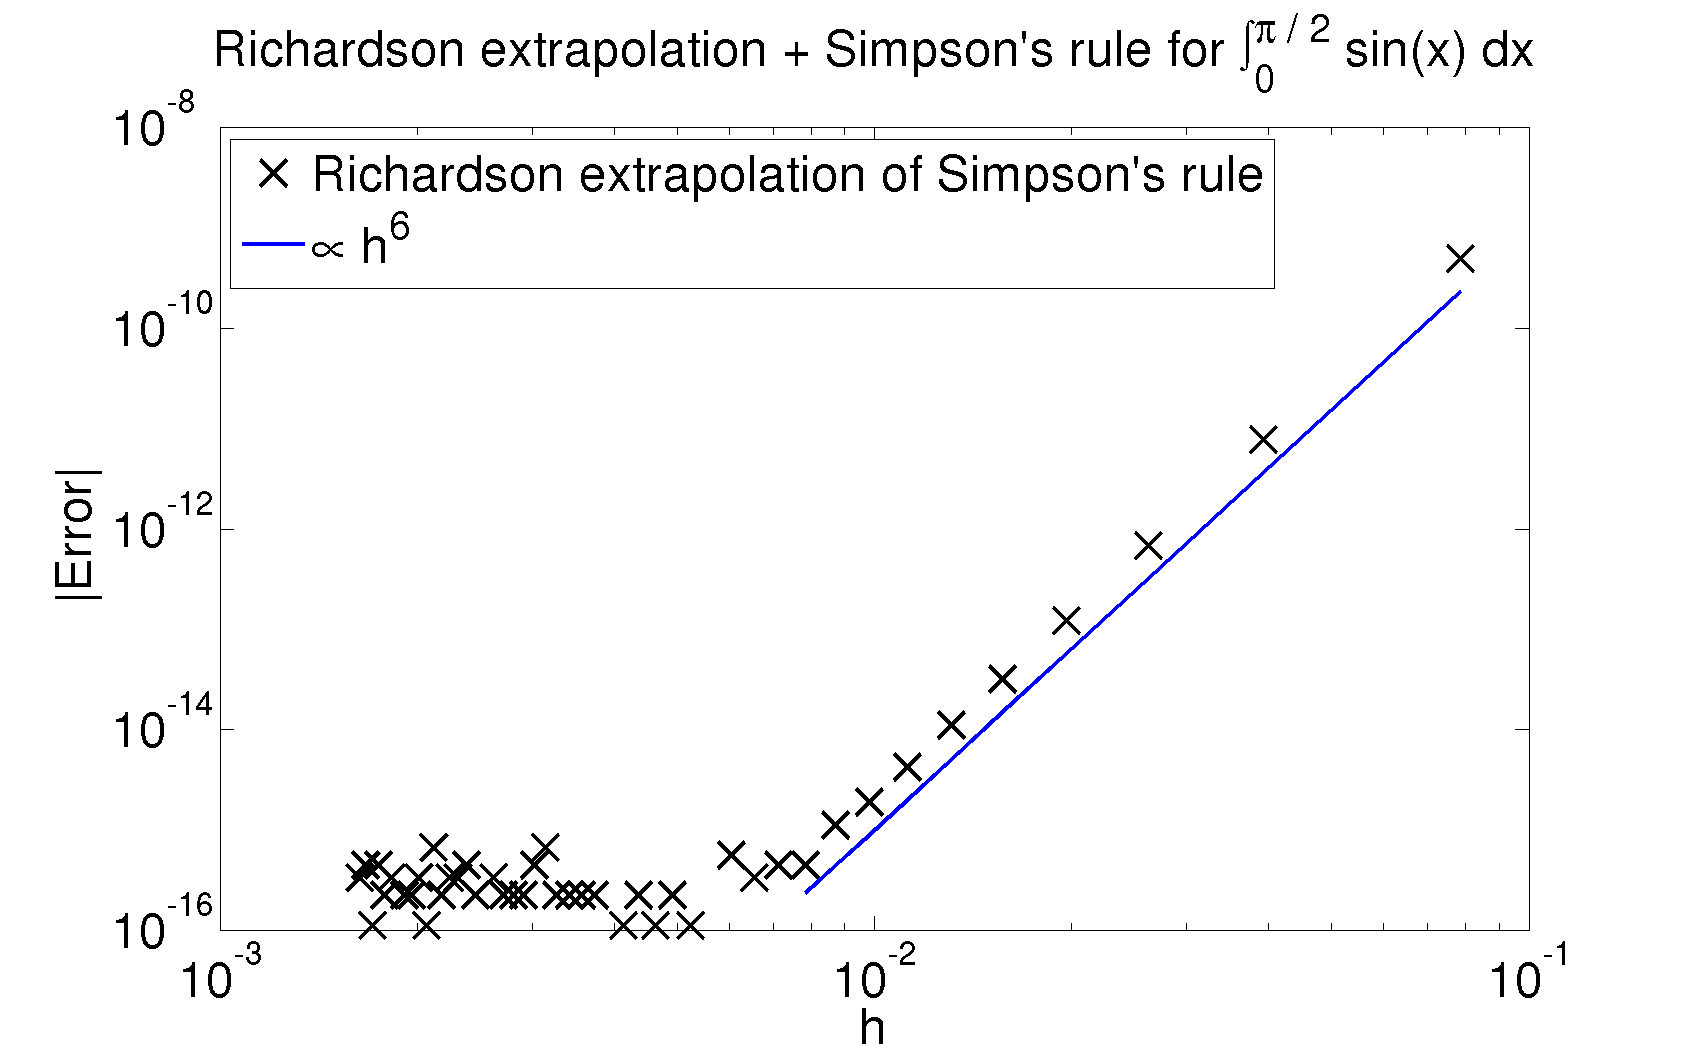
\includegraphics[width=\textwidth]{figures/Richardson1}
      \end{center}
    \end{column}
  \end{columns}

\end{frame}

\section{Summary}

\subsection{Summary}

\begin{frame}
  \frametitle{Summary}

  \begin{itemize}
  \item Simpson's rule is a second order Newton-Cotes formula.
  \item The composite formula is usually employed using equally spaced
    nodes.
  \item The error converges as ${\cal O}(h^4)$.
  \item Richardson extrapolation takes advantage of our knowledge of
    the convergence \emph{rate} to attempt to eliminate the dominant
    error term.
  \end{itemize}

\end{frame}

\end{document}



%%% Local Variables:
%%% mode: latex
%%% TeX-master: t
%%% End:
